\section{Risikoanalyse}
\begin{figure}[H]
	\centering
	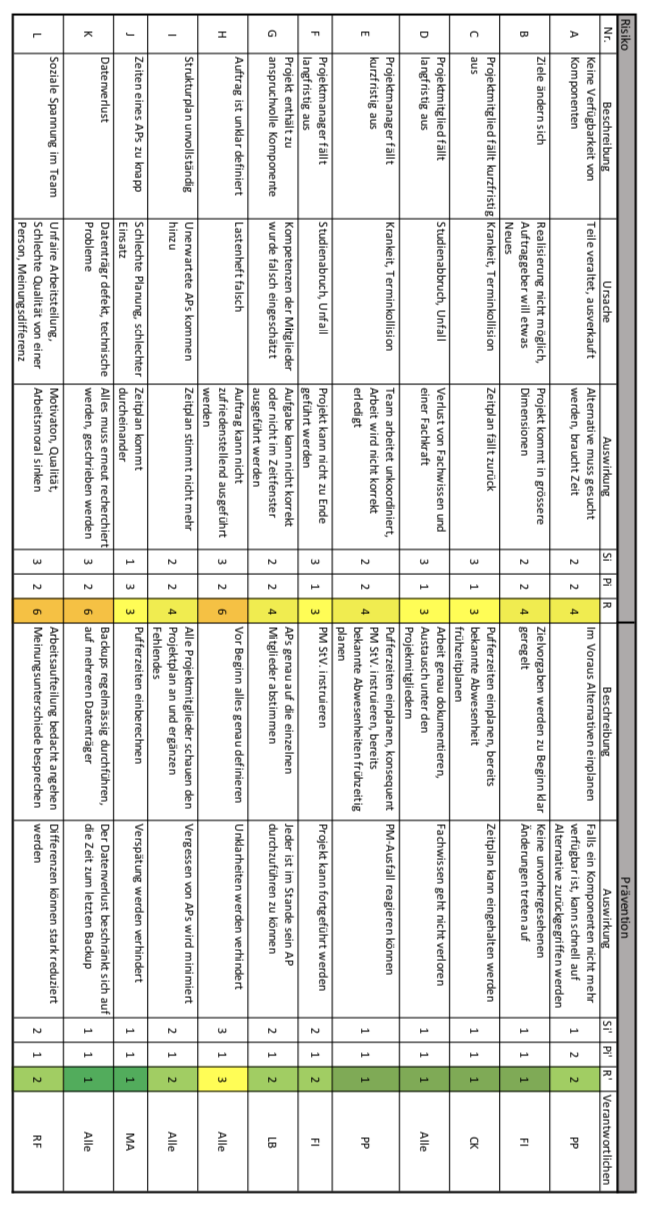
\includegraphics[angle= 180,width=13cm]{Risikoanalyse.png}
	\label{fig:Risikoanalyse}
\end{figure}

\newpage
Um auf Risiken vorbereitet zu sein, macht man eine Risikotabelle. In dieser werden die moeglichen Gefahren aufgelistet und bereits Praeventionsmassnahmen genannt, um sowohl die Eintrittswahrscheinlichkeit(Pi), als auch die Auswirkungen(Si) zu minimieren. Auf der Risikomap werden zudem alle Gefahren mit und ohne Praevention graphisch dargestellt.

\begin{figure}[H]
	\centering
	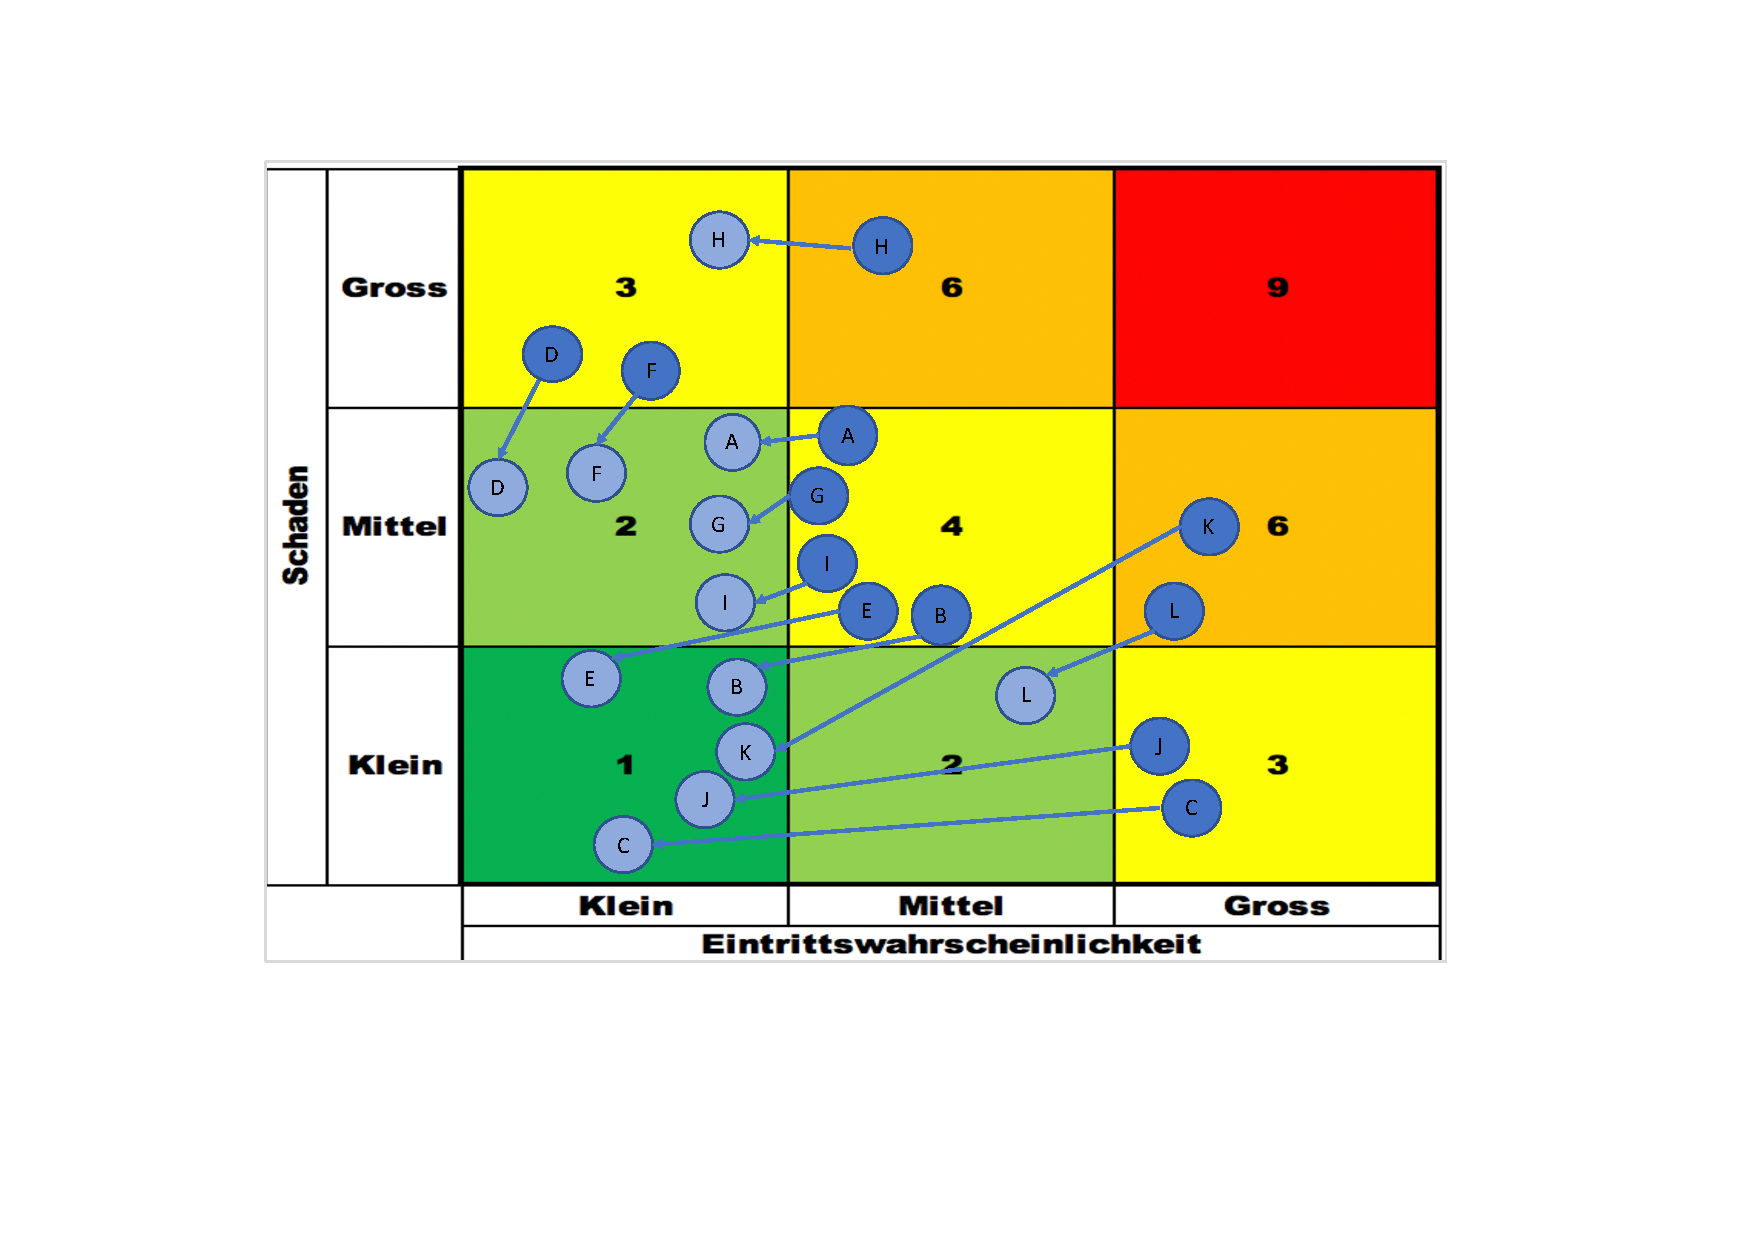
\includegraphics[width=10cm]{Risikotab}
	\label{fig:Risikodiagramm}
\end{figure}

\begin{figure}[H]
	\centering
	\includegraphics[width=10cm]{Risikotabelle}
	\label{fig:Tabelle}
\end{figure}
A 	Keine Verfuegbarkeit von Komponenten \newline 
B 	Ziele aendern sich\newline 
C 	Projektmitglied faellt kurzfristig aus\newline 
D	Projektmitglied faellt langfristig aus\newline 
E 	Projektmanager faelt kurzfristig aus\newline 
F 	Projektmanager faellt langfristig aus\newline 
G	Projekt enthaelt zu anspruchvolle Komponente\newline 
H	Auftrag ist unklar definiert\newline 
I	Strukturplan unvollstaendig\newline 
J	Zeiten eines APs zu knapp\newline 
K	Datenverlust\newline 
L	Soziale Spannung im Team\newline 
